\section{ImMiner Algorithm}
\label{sec:imminer}

We next present an example to explain the major concepts of our ImMiner algorithm and then present a formal definition of the problem addressed by our mining algorithm.

%-----------------------------------------------------------------------
\subsection{Example}

\begin{figure}[t]
\centering
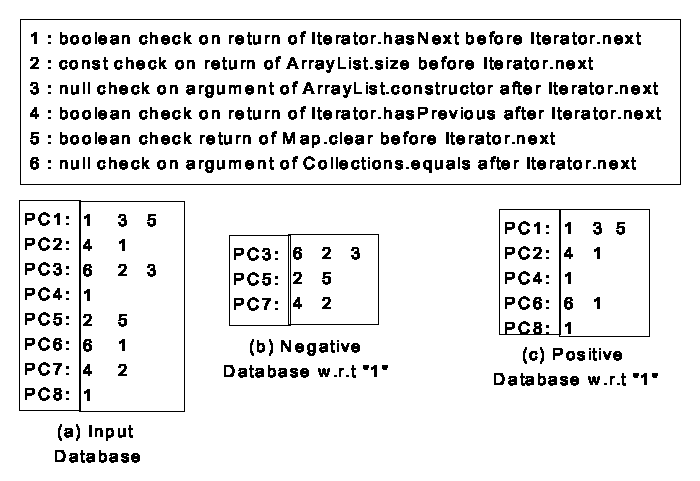
\includegraphics[scale=0.75,clip]{figs/miningex1.eps}\vspace*{-1ex}
\caption{Example for the \CodeIn{Iterator.next} API method used to illustrate our mining algorithm} \label{fig:miningex}
\vspace*{-1ex}
\end{figure}

Figure~\ref{fig:miningex}a shows an input database for applying our mining algorithm, where each row includes the surrounding condition checks (i.e., condition checks before or after an API call) of the same API method from a code example. We refer to each row in the input database as a pattern candidate (PC). For example, PC1 describes that three condition checks are done before and after invoking \CodeIn{Iterator.next}. Given such input database, ImMiner uses two steps for mining alternative patterns of the form ``$P_1$ \textbf{or} $\hat{P_2}$'', where $P_1$ represents ``\CodeIn{boolean check} on the return of \CodeIn{Iterator.hasNext} before \CodeIn{Iterator.next}'' and $P_2$ represents ``\CodeIn{const check} on the return of \CodeIn{ArrayList.size} before \CodeIn{Iterator.next}''.

In Step 1, ImMiner applies frequent itemset mining~\cite{Burdick01mafia} on the input database with a \emph{min\_sup} value, say 0.5. ImMiner identifies a frequent pattern as ``$P_1$: \CodeIn{boolean check} on returns of \CodeIn{Iterator.hasNext} before \CodeIn{Iterator.next}''. In Step 2, ImMiner splits the input database into two databases with respect to $P_1$: negative and positive. The negative database includes all pattern candidates that do not include $P_1$, whereas the positive database includes all pattern candidates that include $P_1$. Figures~\ref{fig:miningex}b and~\ref{fig:miningex}c show the positive and negative databases split with respect to $P_1$. ImMiner next applies frequent itemset mining on the negative database to identify frequent patterns. ImMiner identifies that the frequent pattern in the negative database is  ``$P_2$: \CodeIn{const check} on \CodeIn{ArrayList.size} before \CodeIn{Iterator.next}''. Then ImMiner combines these two patterns to construct an alternative pattern ``$P_1$ \textbf{or} $\hat{P_2}$'', where $P_1$ is a frequent alternative and $P_2$ is an infrequent alternative.

%-----------------------------------------------------------------------
\subsection{Problem Definition}
\label{sec:probdef}

We next present a formal definition of the mining problem targeted by our ImMiner algorithm based on \emph{frequent itemset mining}~\cite{Burdick01mafia}. Although we present our problem definition using frequent itemset mining, our ImMiner algorithm is general and can be used with other mining approaches (such as frequent subsequence mining~\cite{wang:bide}) as well.

Let $M$ = \{$mi_1$, $mi_2$, ..., $mi_k$\} be the set of all possible distinct items. Consider an ItemSet Database $ISD$ 
as \{$is_1$, $is_2$, ...,$is_l$\}, where each itemset $is_j$ includes different sets of elements such as \{$mi_1$, $mi_2$, ..., $mi_a$\} from the set of all possible distinct elements. Consider that a frequent itemset mined from the $ISD$ with a threshold value, say \emph{min\_sup}, is $FIS$ = \{$fi_1$, $fi_2$, ..., $fi_b$\} ($FIS$ denotes Frequent ItemSet). Each $fi_j$ is in the form of \{$mi_1$, $mi_2$, ..., $mi_x$\}. In our context, we refer to $FIS$ as a dominating pattern. The objective of our ImMiner algorithm is to mine imbalanced patterns of the form ``$FIS$ \textbf{or} $\hat{AIS}$'', where $AIS$ is an infrequent alternative pattern of the form \{$ai_1$, $ai_2$, ..., $ai_c$\} ($AIS$ denotes Alternative ItemSet). For each item $fi_i$ $\in$ $FIS$, there can be multiple infrequent alternative items \{$ai_1$, $ai_2$, ..., $ai_d$\} $\in$ $AIS$. The characteristics of each $ai_j$ are such that $ai_j$ is the most frequent in the Negative itemSet Database ($NSD$) and is infrequent in the Positive itemSet Database ($PSD$). Here, $NSD$ represents all itemsets of $ISD$ that do not support $fi_i$ $\in$ $FIS$. We consider that an itemset such as $is_i$ does not support frequent item $fi_i$, if $fi_i$ $\cap$ $is_i$ == $\emptyset$. In contrast, $PSD$ represents all itemsets of $ISD$ that support $fi_i$. We consider that an $is_i$ supports $fi_i$, if $fi_i$ $\cap$ $is_i$ == $fi_i$. Note that $PSD$ $\cap$ $NSD$ == $\emptyset$. However, $PSD$ $\cup$ $NSD$ $\neq$ $ISD$ as there can be some other itemsets $is_j$ that partially support $fi_i$. An $is_j$ is considered as partially supporting $fi_i$, if $fi_i$ $\cap$ $is_i$ $\neq$ $\emptyset$ and $fi_i$ $\cap$ $is_i$ $\neq$ $fi_i$. In our algorithm, we discard such itemsets since these itemsets neither support nor reject the mined items $fi_i$.

In our problem definition, we represent imbalanced patterns as ``$FIS$ \textbf{or} $\hat{AIS}$''. We next present a proof for our representation. Consider that $ai_j \in AIS$ is an infrequent alternative for $fi_i \in FIS$. We represent this pattern as ``R1: $fi_i$ \textbf{or} $\hat{ai_j}$''. Actually, these imbalanced patterns should be of the form ``R2: $fi_i$ \textbf{or} ($\neg$ $fi_i$ \textbf{and} $\hat{ai_j}$)'', since $\hat{ai_j}$ is an infrequent alternative of $fi_i$. However, both representations R1 and R2 are equivalent based on the following proof by considering each alternative as a boolean variable.\\

R2: $fi_i$ \textbf{or} ( $\neg$ $fi_i$ \textbf{and} $\hat{ai_j}$)\\
$\Rightarrow$ ($fi_i$ \textbf{or} $\neg$ $fi_i$) \textbf{and} ($fi_i$ \textbf{or} $\hat{ai_j}$) by distributivity\\
$\Rightarrow$ \CodeIn{True} \textbf{and} ($fi_i$ \textbf{or} $\hat{ai_j}$)\\
$\Rightarrow$ R1: $fi_i$ \textbf{or} $\hat{ai_j}$

Our problem definition also includes a special category of alternative patterns with \emph{only} one alternative in the pattern. This scenario happens when $| FIS |$ = 1 and $AIS = \emptyset$. In summary, our problem definition includes the following three categories of mined patterns defined based on ``$FIS$ \textbf{or} $\hat{AIS}$''.

\begin{itemize}
\item \emph{Balanced:} $AIS = \emptyset$ and $| FIS | > 1$ \\
Example: All alternatives are frequent such as ``$fi_1$ \textbf{or} $fi_2$ \textbf{or} ... \textbf{or} $fi_b$''.
\item \emph{Imbalanced:} $AIS \neq \emptyset$ and $| FIS | \geq 1$ \\
Example: Some alternatives are infrequent such as ``$fi_1$ \textbf{or} $fi_2$ \textbf{or} ... \textbf{or} $fi_b$ \textbf{or} $\hat{ai_1}$ \textbf{or} $\hat{ai_2}$ \textbf{or} ... \textbf{or} $\hat{ai_c}$''.
\item \emph{Single}: $AIS = \emptyset$ and $| FIS |$ = 1\\ Example: Mined pattern includes only one alternative such as ``$fi_i$''.
\end{itemize}

%-----------------------------------------------------------------------
\subsection{Solution}

ImMiner mines all three categories of patterns in two steps. In Step 1, ImMiner 
mines balanced patterns, where all alternatives are frequent. In Step 2,
for each frequent alternative, ImMiner mines infrequent alternatives.

\textbf{Step 1.} ImMiner applies frequent itemset mining such as MAFIA~\cite{Burdick01mafia} on the input database $ISD$.
ImMiner uses a minimum support threshold, say \emph{min\_sup}, for
mining frequent patterns such as $FIS$. ImMiner assigns a support value
given by frequent itemset mining to each mined pattern $FIS$, represented as $SUP(FIS)$.

\textbf{Step 2.} To mine imbalanced patterns for each frequent alternative $fi_i$, ImMiner partitions $ISD$ into two 
groups with respect to the frequent alternative: the negative itemset database ($NSD$) and the positive itemset database ($PSD$). ImMiner partitions the $ISD$ database in such a way that every itemset $NIS$ of $NSD$ does not include any of the items of $fi_i$, whereas every itemset $PIS$ of $PSD$ includes all items of $fi_i$\footnote{Recall that we discard itemsets that partially support $fi_i$}. ImMiner next applies frequent itemset mining on $NSD$ to gather frequent patterns in $NSD$ for each frequent alternative $fi_i$. Consider a mined pattern of $NSD$ as $ai_i$. We next compute a final support value for each infrequent alternative, referred to as $ABS$, using the three formulas below. The notation $\psi(X, Y)$ represents the support of pattern $X$ in database $Y$.

\begin{CodeOut}
\begin{Itemize}
\item $\psi(ai_i, NSD)$ = $\frac{\#\hspace{0.03in}of\hspace{0.03in}pattern candidates\hspace{0.03in}in\hspace{0.03in}NSD\hspace{0.03in}supporting\hspace{0.03in}ai_i}{Total\hspace{0.03in}\#\hspace{0.03in}of\hspace{0.03in}pattern candidates\hspace{0.03in}in\hspace{0.03in}NSD}$\\
\item $\psi(ai_i, PSD)$ = $\frac{\#\hspace{0.03in}of\hspace{0.03in}pattern candidates\hspace{0.03in}in\hspace{0.03in}PSD \hspace{0.03in}supporting\hspace{0.03in}ai_i}{Total\hspace{0.03in}\#\hspace{0.03in}of\hspace{0.03in}pattern candidates\hspace{0.03in}in\hspace{0.03in}PSD}$\\
\item $ABS(ai_i)$ = $\psi(ai_i, NSD)$ - $\psi(ai_i, PSD)$\\
\end{Itemize}
\end{CodeOut}
 
Our formulas assign higher support to those alternative patterns that are frequent in $NSD$ and are infrequent in $PSD$. The rationale behind these formulas is that \emph{only} such patterns can be treated as infrequent alternative patterns for $FIS$. Similar to \emph{min\_sup} for mining $FIS$, we use another user-defined threshold such as \emph{alt\_sup} for mining infrequent alternative patterns. Based on the number of elements in $FIS$ and $AIS$, ImMiner assigns category types
to mined patterns.

 